\documentclass[14pt]{extarticle}
\usepackage[T1]{fontenc}
\usepackage[default]{sourcesanspro}
\usepackage[letterpaper,top=0.75in,bottom=0.75in,left=0.65in,right=0.65in,
  headheight=18pt,headsep=0.28in,footskip=0.45in]{geometry}
\usepackage{tikz}
\usepackage{fancyhdr}
\usepackage[none]{hyphenat}
\usepackage{ragged2e}
\definecolor{cube}{RGB}{176,204,236}
\definecolor{folder}{RGB}{240,218,166}
\pagestyle{fancy}
\fancyhf{}
\fancyhead[L]{Week 5 / Tower cities / Grades 4--5}
\fancyfoot[L]{Bellingham Math Circle / Week 5 / F05-U-v4}
\fancyfoot[R]{\thepage}
\renewcommand{\headrulewidth}{0.4pt}
\renewcommand{\footrulewidth}{0pt}
\setlength{\parindent}{0pt}
\setlength{\parskip}{0pt}
\raggedbottom
\RaggedRight
\newcommand{\prob}[1]{\textbf{Problem #1:}\ }
\begin{document}
Look along a row of towers from one end, with your eye down at the table about a foot away. You see a tower when it is taller than every tower in front of it.
\par\vspace{0.6cm}
\begin{minipage}{\linewidth}\RaggedRight
\prob{1}Use towers of 1, 2, 3, and 4 cubes. For each card, find a row that shows the left number from the left end and the right number from the right end, and write the heights of the row on the card. If no row can, explain why.
\vspace*{0.2cm}
\begin{center}
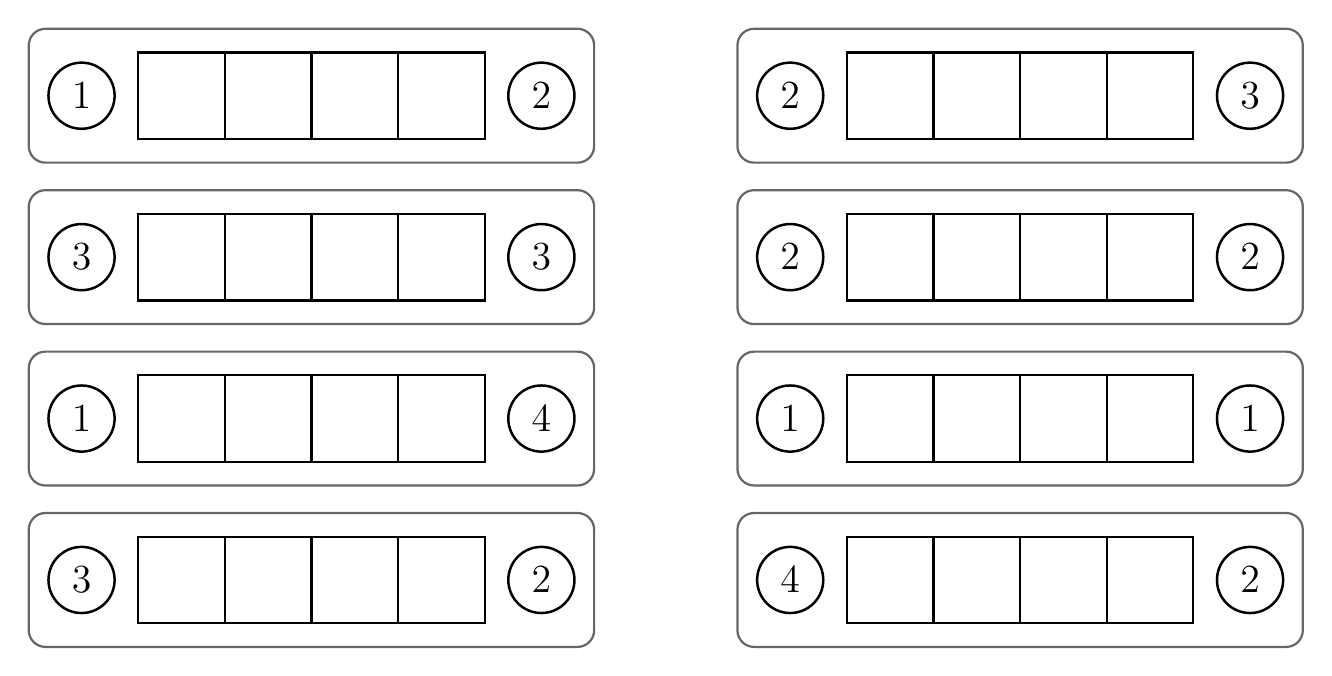
\begin{tikzpicture}
\begin{scope}[shift={(0.000,0.000)}]
\draw[line width=0.8pt] (0.000,0) rectangle (1.100,1.100);
\draw[line width=0.8pt] (1.100,0) rectangle (2.200,1.100);
\draw[line width=0.8pt] (2.200,0) rectangle (3.300,1.100);
\draw[line width=0.8pt] (3.300,0) rectangle (4.400,1.100);
\draw[line width=0.9pt] (-0.720,0.550) circle (0.420);
\node at (-0.720,0.550) {\Large 1};
\draw[line width=0.9pt] (5.120,0.550) circle (0.420);
\node at (5.120,0.550) {\Large 2};
\draw[rounded corners=6pt, line width=0.8pt, black!60] (-1.390,-0.3) rectangle (5.790,1.400);
\end{scope}
\begin{scope}[shift={(9.000,0.000)}]
\draw[line width=0.8pt] (0.000,0) rectangle (1.100,1.100);
\draw[line width=0.8pt] (1.100,0) rectangle (2.200,1.100);
\draw[line width=0.8pt] (2.200,0) rectangle (3.300,1.100);
\draw[line width=0.8pt] (3.300,0) rectangle (4.400,1.100);
\draw[line width=0.9pt] (-0.720,0.550) circle (0.420);
\node at (-0.720,0.550) {\Large 2};
\draw[line width=0.9pt] (5.120,0.550) circle (0.420);
\node at (5.120,0.550) {\Large 3};
\draw[rounded corners=6pt, line width=0.8pt, black!60] (-1.390,-0.3) rectangle (5.790,1.400);
\end{scope}
\begin{scope}[shift={(0.000,-2.050)}]
\draw[line width=0.8pt] (0.000,0) rectangle (1.100,1.100);
\draw[line width=0.8pt] (1.100,0) rectangle (2.200,1.100);
\draw[line width=0.8pt] (2.200,0) rectangle (3.300,1.100);
\draw[line width=0.8pt] (3.300,0) rectangle (4.400,1.100);
\draw[line width=0.9pt] (-0.720,0.550) circle (0.420);
\node at (-0.720,0.550) {\Large 3};
\draw[line width=0.9pt] (5.120,0.550) circle (0.420);
\node at (5.120,0.550) {\Large 3};
\draw[rounded corners=6pt, line width=0.8pt, black!60] (-1.390,-0.3) rectangle (5.790,1.400);
\end{scope}
\begin{scope}[shift={(9.000,-2.050)}]
\draw[line width=0.8pt] (0.000,0) rectangle (1.100,1.100);
\draw[line width=0.8pt] (1.100,0) rectangle (2.200,1.100);
\draw[line width=0.8pt] (2.200,0) rectangle (3.300,1.100);
\draw[line width=0.8pt] (3.300,0) rectangle (4.400,1.100);
\draw[line width=0.9pt] (-0.720,0.550) circle (0.420);
\node at (-0.720,0.550) {\Large 2};
\draw[line width=0.9pt] (5.120,0.550) circle (0.420);
\node at (5.120,0.550) {\Large 2};
\draw[rounded corners=6pt, line width=0.8pt, black!60] (-1.390,-0.3) rectangle (5.790,1.400);
\end{scope}
\begin{scope}[shift={(0.000,-4.100)}]
\draw[line width=0.8pt] (0.000,0) rectangle (1.100,1.100);
\draw[line width=0.8pt] (1.100,0) rectangle (2.200,1.100);
\draw[line width=0.8pt] (2.200,0) rectangle (3.300,1.100);
\draw[line width=0.8pt] (3.300,0) rectangle (4.400,1.100);
\draw[line width=0.9pt] (-0.720,0.550) circle (0.420);
\node at (-0.720,0.550) {\Large 1};
\draw[line width=0.9pt] (5.120,0.550) circle (0.420);
\node at (5.120,0.550) {\Large 4};
\draw[rounded corners=6pt, line width=0.8pt, black!60] (-1.390,-0.3) rectangle (5.790,1.400);
\end{scope}
\begin{scope}[shift={(9.000,-4.100)}]
\draw[line width=0.8pt] (0.000,0) rectangle (1.100,1.100);
\draw[line width=0.8pt] (1.100,0) rectangle (2.200,1.100);
\draw[line width=0.8pt] (2.200,0) rectangle (3.300,1.100);
\draw[line width=0.8pt] (3.300,0) rectangle (4.400,1.100);
\draw[line width=0.9pt] (-0.720,0.550) circle (0.420);
\node at (-0.720,0.550) {\Large 1};
\draw[line width=0.9pt] (5.120,0.550) circle (0.420);
\node at (5.120,0.550) {\Large 1};
\draw[rounded corners=6pt, line width=0.8pt, black!60] (-1.390,-0.3) rectangle (5.790,1.400);
\end{scope}
\begin{scope}[shift={(0.000,-6.150)}]
\draw[line width=0.8pt] (0.000,0) rectangle (1.100,1.100);
\draw[line width=0.8pt] (1.100,0) rectangle (2.200,1.100);
\draw[line width=0.8pt] (2.200,0) rectangle (3.300,1.100);
\draw[line width=0.8pt] (3.300,0) rectangle (4.400,1.100);
\draw[line width=0.9pt] (-0.720,0.550) circle (0.420);
\node at (-0.720,0.550) {\Large 3};
\draw[line width=0.9pt] (5.120,0.550) circle (0.420);
\node at (5.120,0.550) {\Large 2};
\draw[rounded corners=6pt, line width=0.8pt, black!60] (-1.390,-0.3) rectangle (5.790,1.400);
\end{scope}
\begin{scope}[shift={(9.000,-6.150)}]
\draw[line width=0.8pt] (0.000,0) rectangle (1.100,1.100);
\draw[line width=0.8pt] (1.100,0) rectangle (2.200,1.100);
\draw[line width=0.8pt] (2.200,0) rectangle (3.300,1.100);
\draw[line width=0.8pt] (3.300,0) rectangle (4.400,1.100);
\draw[line width=0.9pt] (-0.720,0.550) circle (0.420);
\node at (-0.720,0.550) {\Large 4};
\draw[line width=0.9pt] (5.120,0.550) circle (0.420);
\node at (5.120,0.550) {\Large 2};
\draw[rounded corners=6pt, line width=0.8pt, black!60] (-1.390,-0.3) rectangle (5.790,1.400);
\end{scope}
\end{tikzpicture}
\end{center}
\vspace*{3.0cm}
\end{minipage}
\par\vspace{0.75cm}
\newpage
\begin{minipage}{\linewidth}\RaggedRight
\prob{2}Build sixteen towers on this grid with your 40 cubes, one tower on each square, so that every row and every column has one tower of each height 1, 2, 3, and 4. Towers placed like this make a city. In the boxes around the grid, write how many towers you see from each end of every row and every column, and write the heights in the grid.
\vspace*{0.3cm}
\begin{center}
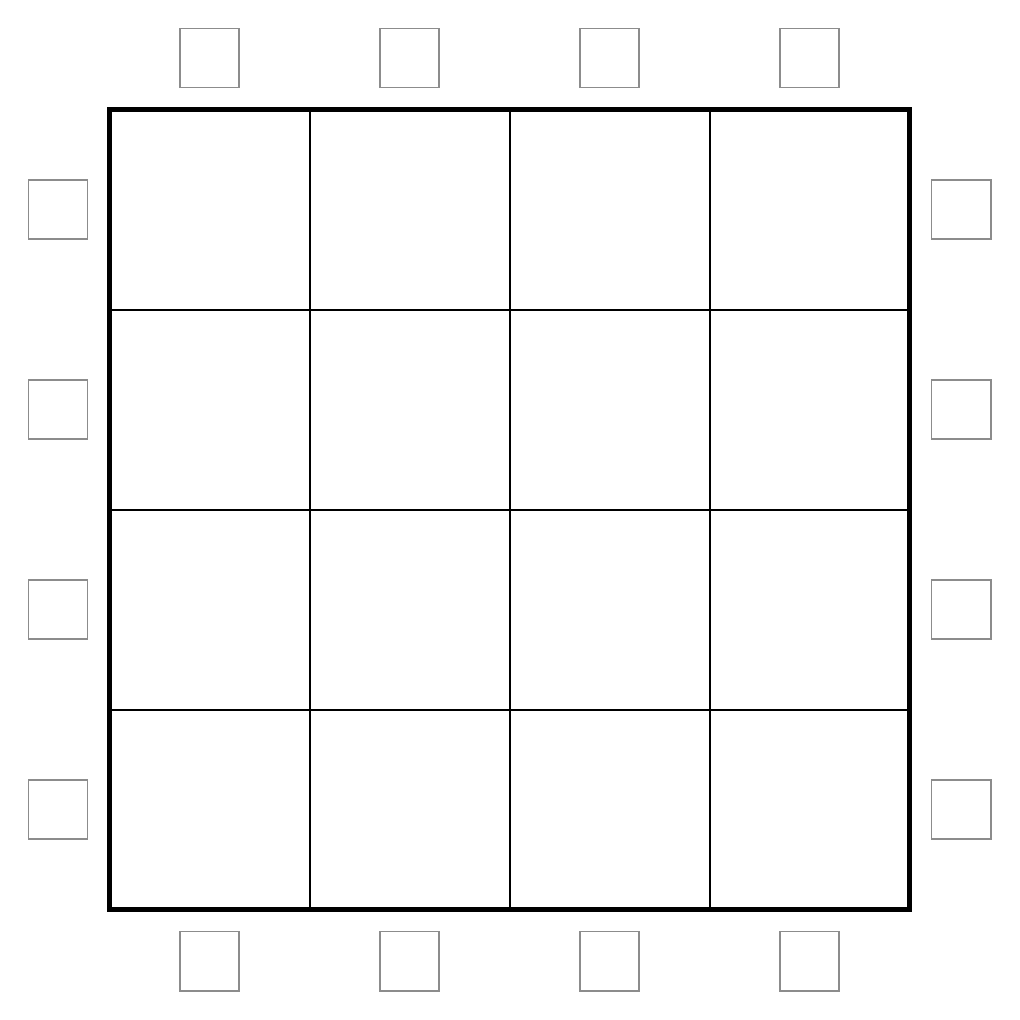
\begin{tikzpicture}
\begin{scope}[shift={(0.000,0.000)}]
\draw[line width=0.7pt] (2.540,0) -- (2.540,10.160);
\draw[line width=0.7pt] (0,2.540) -- (10.160,2.540);
\draw[line width=0.7pt] (5.080,0) -- (5.080,10.160);
\draw[line width=0.7pt] (0,5.080) -- (10.160,5.080);
\draw[line width=0.7pt] (7.620,0) -- (7.620,10.160);
\draw[line width=0.7pt] (0,7.620) -- (10.160,7.620);
\draw[line width=1.6pt] (0,0) rectangle (10.160,10.160);
\draw[black!45, line width=0.6pt] (0.895,10.440) rectangle (1.645,11.190);
\draw[black!45, line width=0.6pt] (3.435,10.440) rectangle (4.185,11.190);
\draw[black!45, line width=0.6pt] (5.975,10.440) rectangle (6.725,11.190);
\draw[black!45, line width=0.6pt] (8.515,10.440) rectangle (9.265,11.190);
\draw[black!45, line width=0.6pt] (0.895,-1.030) rectangle (1.645,-0.280);
\draw[black!45, line width=0.6pt] (3.435,-1.030) rectangle (4.185,-0.280);
\draw[black!45, line width=0.6pt] (5.975,-1.030) rectangle (6.725,-0.280);
\draw[black!45, line width=0.6pt] (8.515,-1.030) rectangle (9.265,-0.280);
\draw[black!45, line width=0.6pt] (-1.030,8.515) rectangle (-0.280,9.265);
\draw[black!45, line width=0.6pt] (-1.030,5.975) rectangle (-0.280,6.725);
\draw[black!45, line width=0.6pt] (-1.030,3.435) rectangle (-0.280,4.185);
\draw[black!45, line width=0.6pt] (-1.030,0.895) rectangle (-0.280,1.645);
\draw[black!45, line width=0.6pt] (10.440,8.515) rectangle (11.190,9.265);
\draw[black!45, line width=0.6pt] (10.440,5.975) rectangle (11.190,6.725);
\draw[black!45, line width=0.6pt] (10.440,3.435) rectangle (11.190,4.185);
\draw[black!45, line width=0.6pt] (10.440,0.895) rectangle (11.190,1.645);
\end{scope}
\end{tikzpicture}
\end{center}
\end{minipage}
\par\vspace{0.75cm}
\newpage
\begin{minipage}{\linewidth}\RaggedRight
\prob{3}Find the city that fits the numbers around each grid, and write its heights in the grid.
\vspace*{0.3cm}
\begin{center}
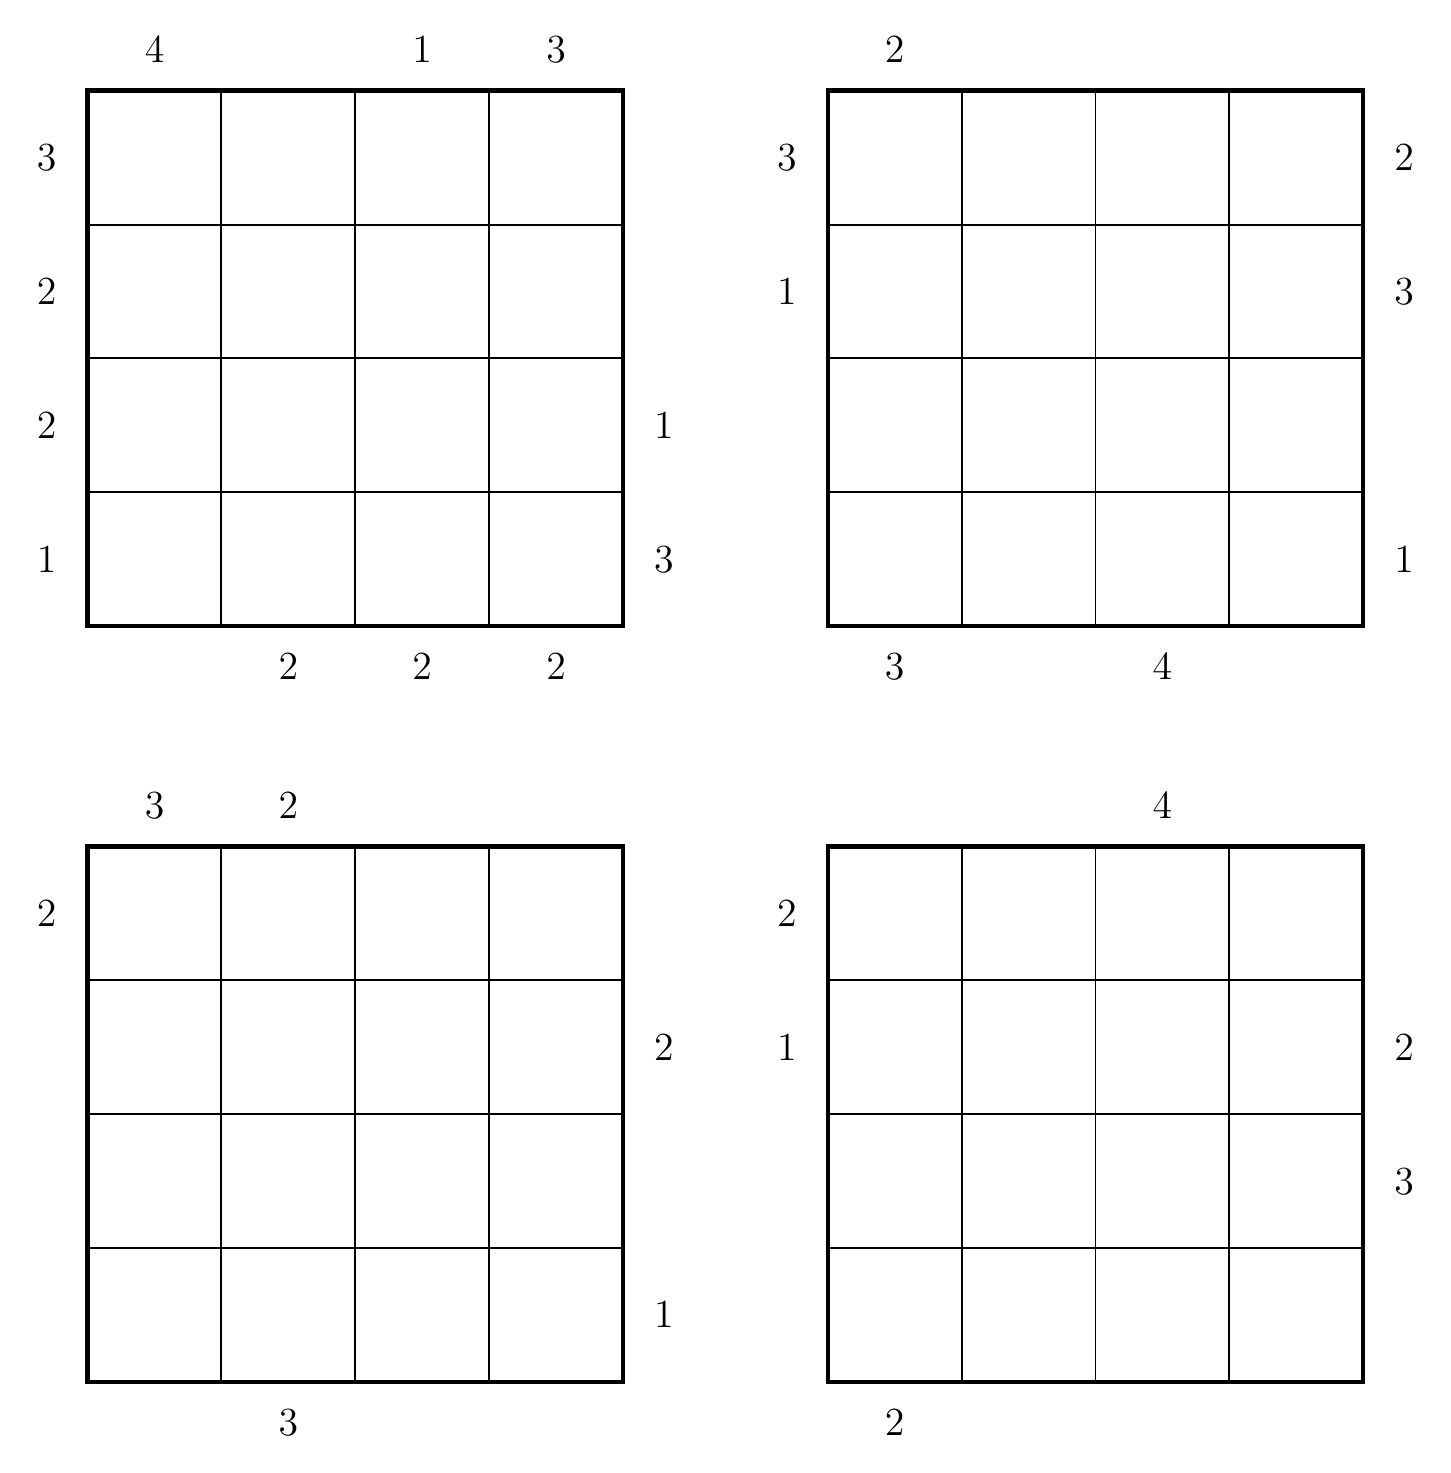
\begin{tikzpicture}
\begin{scope}[shift={(0.000,0.000)}]
\draw[line width=0.7pt] (1.700,0) -- (1.700,6.800);
\draw[line width=0.7pt] (0,1.700) -- (6.800,1.700);
\draw[line width=0.7pt] (3.400,0) -- (3.400,6.800);
\draw[line width=0.7pt] (0,3.400) -- (6.800,3.400);
\draw[line width=0.7pt] (5.100,0) -- (5.100,6.800);
\draw[line width=0.7pt] (0,5.100) -- (6.800,5.100);
\draw[line width=1.6pt] (0,0) rectangle (6.800,6.800);
\node at (0.850,7.320) {\Large 4};
\node at (4.250,7.320) {\Large 1};
\node at (5.950,7.320) {\Large 3};
\node at (2.550,-0.520) {\Large 2};
\node at (4.250,-0.520) {\Large 2};
\node at (5.950,-0.520) {\Large 2};
\node at (-0.520,5.950) {\Large 3};
\node at (-0.520,4.250) {\Large 2};
\node at (-0.520,2.550) {\Large 2};
\node at (-0.520,0.850) {\Large 1};
\node at (7.320,2.550) {\Large 1};
\node at (7.320,0.850) {\Large 3};
\end{scope}
\begin{scope}[shift={(9.400,0.000)}]
\draw[line width=0.7pt] (1.700,0) -- (1.700,6.800);
\draw[line width=0.7pt] (0,1.700) -- (6.800,1.700);
\draw[line width=0.7pt] (3.400,0) -- (3.400,6.800);
\draw[line width=0.7pt] (0,3.400) -- (6.800,3.400);
\draw[line width=0.7pt] (5.100,0) -- (5.100,6.800);
\draw[line width=0.7pt] (0,5.100) -- (6.800,5.100);
\draw[line width=1.6pt] (0,0) rectangle (6.800,6.800);
\node at (0.850,7.320) {\Large 2};
\node at (0.850,-0.520) {\Large 3};
\node at (4.250,-0.520) {\Large 4};
\node at (-0.520,5.950) {\Large 3};
\node at (-0.520,4.250) {\Large 1};
\node at (7.320,5.950) {\Large 2};
\node at (7.320,4.250) {\Large 3};
\node at (7.320,0.850) {\Large 1};
\end{scope}
\begin{scope}[shift={(0.000,-9.600)}]
\draw[line width=0.7pt] (1.700,0) -- (1.700,6.800);
\draw[line width=0.7pt] (0,1.700) -- (6.800,1.700);
\draw[line width=0.7pt] (3.400,0) -- (3.400,6.800);
\draw[line width=0.7pt] (0,3.400) -- (6.800,3.400);
\draw[line width=0.7pt] (5.100,0) -- (5.100,6.800);
\draw[line width=0.7pt] (0,5.100) -- (6.800,5.100);
\draw[line width=1.6pt] (0,0) rectangle (6.800,6.800);
\node at (0.850,7.320) {\Large 3};
\node at (2.550,7.320) {\Large 2};
\node at (2.550,-0.520) {\Large 3};
\node at (-0.520,5.950) {\Large 2};
\node at (7.320,4.250) {\Large 2};
\node at (7.320,0.850) {\Large 1};
\end{scope}
\begin{scope}[shift={(9.400,-9.600)}]
\draw[line width=0.7pt] (1.700,0) -- (1.700,6.800);
\draw[line width=0.7pt] (0,1.700) -- (6.800,1.700);
\draw[line width=0.7pt] (3.400,0) -- (3.400,6.800);
\draw[line width=0.7pt] (0,3.400) -- (6.800,3.400);
\draw[line width=0.7pt] (5.100,0) -- (5.100,6.800);
\draw[line width=0.7pt] (0,5.100) -- (6.800,5.100);
\draw[line width=1.6pt] (0,0) rectangle (6.800,6.800);
\node at (4.250,7.320) {\Large 4};
\node at (0.850,-0.520) {\Large 2};
\node at (-0.520,5.950) {\Large 2};
\node at (-0.520,4.250) {\Large 1};
\node at (7.320,4.250) {\Large 2};
\node at (7.320,2.550) {\Large 3};
\end{scope}
\end{tikzpicture}
\end{center}
\end{minipage}
\par\vspace{0.75cm}
\newpage
\vspace*{0.3cm}
\begin{center}
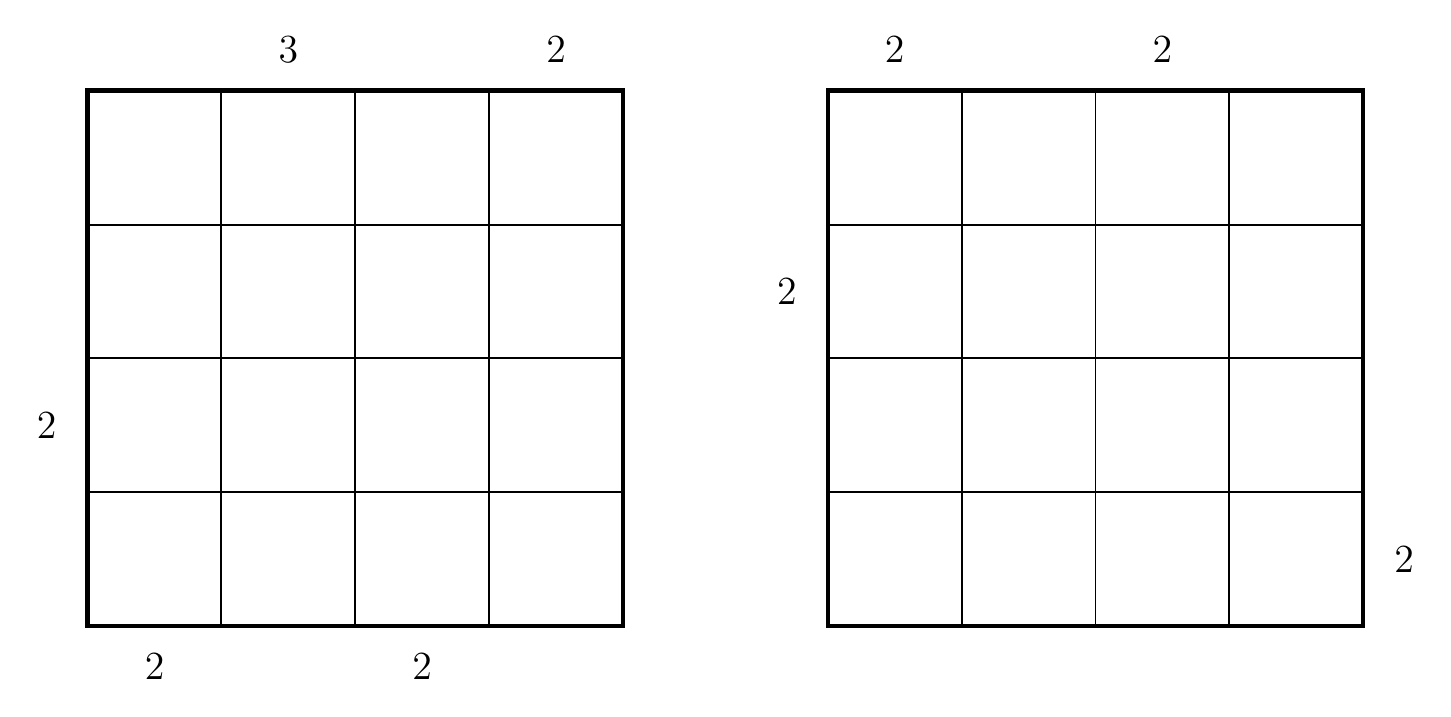
\begin{tikzpicture}
\begin{scope}[shift={(0.000,0.000)}]
\draw[line width=0.7pt] (1.700,0) -- (1.700,6.800);
\draw[line width=0.7pt] (0,1.700) -- (6.800,1.700);
\draw[line width=0.7pt] (3.400,0) -- (3.400,6.800);
\draw[line width=0.7pt] (0,3.400) -- (6.800,3.400);
\draw[line width=0.7pt] (5.100,0) -- (5.100,6.800);
\draw[line width=0.7pt] (0,5.100) -- (6.800,5.100);
\draw[line width=1.6pt] (0,0) rectangle (6.800,6.800);
\node at (2.550,7.320) {\Large 3};
\node at (5.950,7.320) {\Large 2};
\node at (0.850,-0.520) {\Large 2};
\node at (4.250,-0.520) {\Large 2};
\node at (-0.520,2.550) {\Large 2};
\end{scope}
\begin{scope}[shift={(9.400,0.000)}]
\draw[line width=0.7pt] (1.700,0) -- (1.700,6.800);
\draw[line width=0.7pt] (0,1.700) -- (6.800,1.700);
\draw[line width=0.7pt] (3.400,0) -- (3.400,6.800);
\draw[line width=0.7pt] (0,3.400) -- (6.800,3.400);
\draw[line width=0.7pt] (5.100,0) -- (5.100,6.800);
\draw[line width=0.7pt] (0,5.100) -- (6.800,5.100);
\draw[line width=1.6pt] (0,0) rectangle (6.800,6.800);
\node at (0.850,7.320) {\Large 2};
\node at (4.250,7.320) {\Large 2};
\node at (-0.520,4.250) {\Large 2};
\node at (7.320,0.850) {\Large 2};
\end{scope}
\end{tikzpicture}
\end{center}
\newpage
\begin{minipage}{\linewidth}\RaggedRight
\prob{4}More than one city fits the numbers around this grid. Find every city that fits. Then write one more number around the grid so that only one of your cities fits.
\vspace*{0.2cm}
\begin{center}
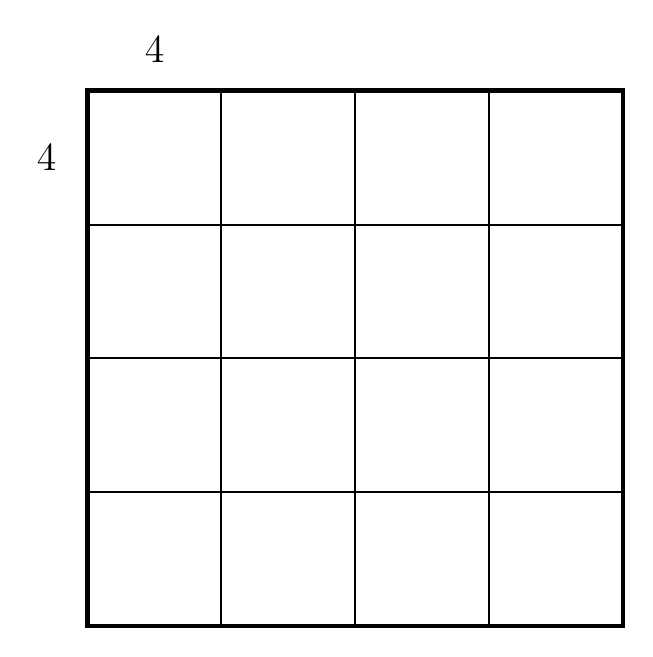
\begin{tikzpicture}
\draw[line width=0.7pt] (1.700,0) -- (1.700,6.800);
\draw[line width=0.7pt] (0,1.700) -- (6.800,1.700);
\draw[line width=0.7pt] (3.400,0) -- (3.400,6.800);
\draw[line width=0.7pt] (0,3.400) -- (6.800,3.400);
\draw[line width=0.7pt] (5.100,0) -- (5.100,6.800);
\draw[line width=0.7pt] (0,5.100) -- (6.800,5.100);
\draw[line width=1.6pt] (0,0) rectangle (6.800,6.800);
\node at (0.850,7.320) {\Large 4};
\node at (-0.520,5.950) {\Large 4};
\end{tikzpicture}
\end{center}
\vspace*{0.3cm}
\begin{center}
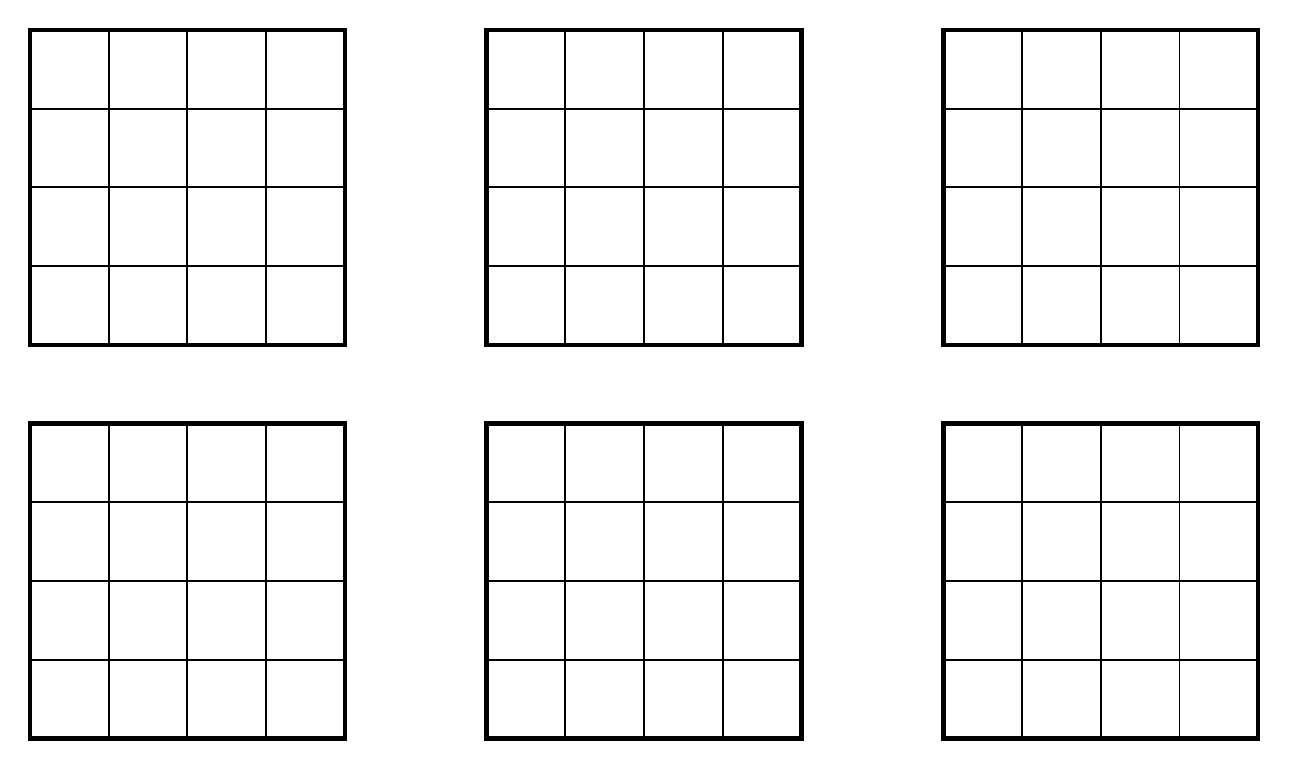
\begin{tikzpicture}
\begin{scope}[shift={(0.000,0.000)}]
\draw[line width=0.7pt] (1.000,0) -- (1.000,4.000);
\draw[line width=0.7pt] (0,1.000) -- (4.000,1.000);
\draw[line width=0.7pt] (2.000,0) -- (2.000,4.000);
\draw[line width=0.7pt] (0,2.000) -- (4.000,2.000);
\draw[line width=0.7pt] (3.000,0) -- (3.000,4.000);
\draw[line width=0.7pt] (0,3.000) -- (4.000,3.000);
\draw[line width=1.6pt] (0,0) rectangle (4.000,4.000);
\end{scope}
\begin{scope}[shift={(5.800,0.000)}]
\draw[line width=0.7pt] (1.000,0) -- (1.000,4.000);
\draw[line width=0.7pt] (0,1.000) -- (4.000,1.000);
\draw[line width=0.7pt] (2.000,0) -- (2.000,4.000);
\draw[line width=0.7pt] (0,2.000) -- (4.000,2.000);
\draw[line width=0.7pt] (3.000,0) -- (3.000,4.000);
\draw[line width=0.7pt] (0,3.000) -- (4.000,3.000);
\draw[line width=1.6pt] (0,0) rectangle (4.000,4.000);
\end{scope}
\begin{scope}[shift={(11.600,0.000)}]
\draw[line width=0.7pt] (1.000,0) -- (1.000,4.000);
\draw[line width=0.7pt] (0,1.000) -- (4.000,1.000);
\draw[line width=0.7pt] (2.000,0) -- (2.000,4.000);
\draw[line width=0.7pt] (0,2.000) -- (4.000,2.000);
\draw[line width=0.7pt] (3.000,0) -- (3.000,4.000);
\draw[line width=0.7pt] (0,3.000) -- (4.000,3.000);
\draw[line width=1.6pt] (0,0) rectangle (4.000,4.000);
\end{scope}
\begin{scope}[shift={(0.000,-5.000)}]
\draw[line width=0.7pt] (1.000,0) -- (1.000,4.000);
\draw[line width=0.7pt] (0,1.000) -- (4.000,1.000);
\draw[line width=0.7pt] (2.000,0) -- (2.000,4.000);
\draw[line width=0.7pt] (0,2.000) -- (4.000,2.000);
\draw[line width=0.7pt] (3.000,0) -- (3.000,4.000);
\draw[line width=0.7pt] (0,3.000) -- (4.000,3.000);
\draw[line width=1.6pt] (0,0) rectangle (4.000,4.000);
\end{scope}
\begin{scope}[shift={(5.800,-5.000)}]
\draw[line width=0.7pt] (1.000,0) -- (1.000,4.000);
\draw[line width=0.7pt] (0,1.000) -- (4.000,1.000);
\draw[line width=0.7pt] (2.000,0) -- (2.000,4.000);
\draw[line width=0.7pt] (0,2.000) -- (4.000,2.000);
\draw[line width=0.7pt] (3.000,0) -- (3.000,4.000);
\draw[line width=0.7pt] (0,3.000) -- (4.000,3.000);
\draw[line width=1.6pt] (0,0) rectangle (4.000,4.000);
\end{scope}
\begin{scope}[shift={(11.600,-5.000)}]
\draw[line width=0.7pt] (1.000,0) -- (1.000,4.000);
\draw[line width=0.7pt] (0,1.000) -- (4.000,1.000);
\draw[line width=0.7pt] (2.000,0) -- (2.000,4.000);
\draw[line width=0.7pt] (0,2.000) -- (4.000,2.000);
\draw[line width=0.7pt] (3.000,0) -- (3.000,4.000);
\draw[line width=0.7pt] (0,3.000) -- (4.000,3.000);
\draw[line width=1.6pt] (0,0) rectangle (4.000,4.000);
\end{scope}
\end{tikzpicture}
\end{center}
\end{minipage}
\par\vspace{0.75cm}
\newpage
\begin{minipage}{\linewidth}\RaggedRight
\prob{5}Build a city behind a folder, out of your partner's sight. Write some of its numbers around an empty grid so that your city is the only one that fits, using as few numbers as you can. Your partner solves the puzzle and then tries to find a second city that fits the same numbers.
\vspace*{0.2cm}
\begin{center}
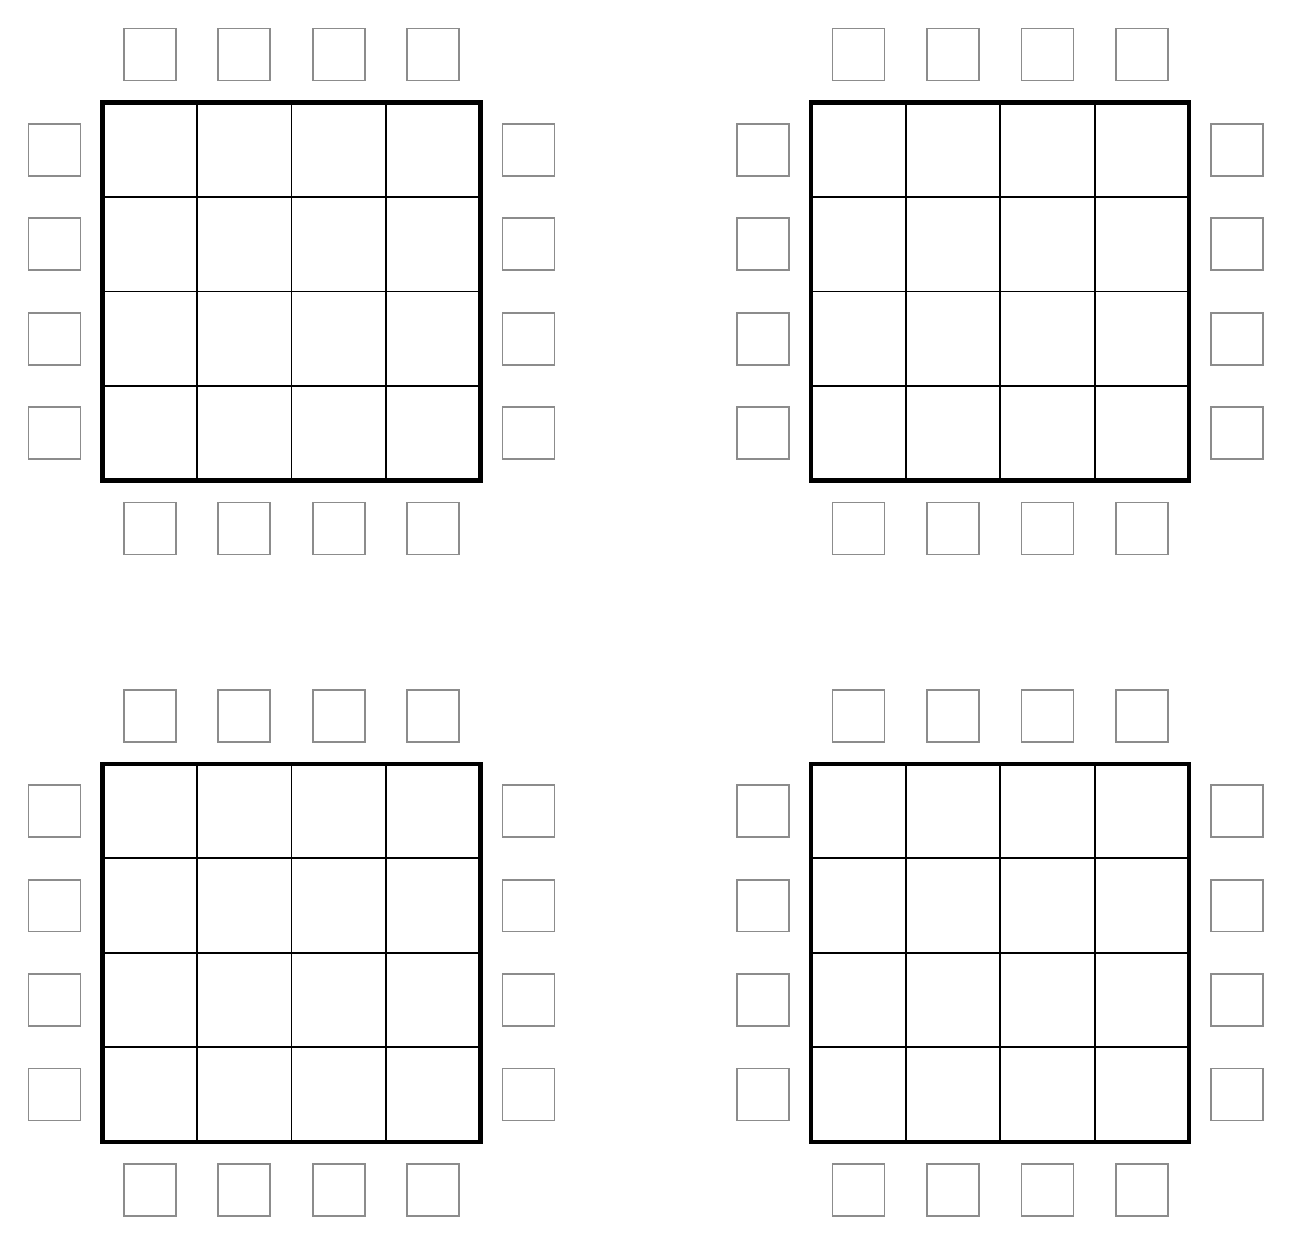
\begin{tikzpicture}
\begin{scope}[shift={(0.000,0.000)}]
\draw[line width=0.7pt] (1.200,0) -- (1.200,4.800);
\draw[line width=0.7pt] (0,1.200) -- (4.800,1.200);
\draw[line width=0.7pt] (2.400,0) -- (2.400,4.800);
\draw[line width=0.7pt] (0,2.400) -- (4.800,2.400);
\draw[line width=0.7pt] (3.600,0) -- (3.600,4.800);
\draw[line width=0.7pt] (0,3.600) -- (4.800,3.600);
\draw[line width=1.6pt] (0,0) rectangle (4.800,4.800);
\draw[black!45, line width=0.6pt] (0.270,5.080) rectangle (0.930,5.740);
\draw[black!45, line width=0.6pt] (1.470,5.080) rectangle (2.130,5.740);
\draw[black!45, line width=0.6pt] (2.670,5.080) rectangle (3.330,5.740);
\draw[black!45, line width=0.6pt] (3.870,5.080) rectangle (4.530,5.740);
\draw[black!45, line width=0.6pt] (0.270,-0.940) rectangle (0.930,-0.280);
\draw[black!45, line width=0.6pt] (1.470,-0.940) rectangle (2.130,-0.280);
\draw[black!45, line width=0.6pt] (2.670,-0.940) rectangle (3.330,-0.280);
\draw[black!45, line width=0.6pt] (3.870,-0.940) rectangle (4.530,-0.280);
\draw[black!45, line width=0.6pt] (-0.940,3.870) rectangle (-0.280,4.530);
\draw[black!45, line width=0.6pt] (-0.940,2.670) rectangle (-0.280,3.330);
\draw[black!45, line width=0.6pt] (-0.940,1.470) rectangle (-0.280,2.130);
\draw[black!45, line width=0.6pt] (-0.940,0.270) rectangle (-0.280,0.930);
\draw[black!45, line width=0.6pt] (5.080,3.870) rectangle (5.740,4.530);
\draw[black!45, line width=0.6pt] (5.080,2.670) rectangle (5.740,3.330);
\draw[black!45, line width=0.6pt] (5.080,1.470) rectangle (5.740,2.130);
\draw[black!45, line width=0.6pt] (5.080,0.270) rectangle (5.740,0.930);
\end{scope}
\begin{scope}[shift={(9.000,0.000)}]
\draw[line width=0.7pt] (1.200,0) -- (1.200,4.800);
\draw[line width=0.7pt] (0,1.200) -- (4.800,1.200);
\draw[line width=0.7pt] (2.400,0) -- (2.400,4.800);
\draw[line width=0.7pt] (0,2.400) -- (4.800,2.400);
\draw[line width=0.7pt] (3.600,0) -- (3.600,4.800);
\draw[line width=0.7pt] (0,3.600) -- (4.800,3.600);
\draw[line width=1.6pt] (0,0) rectangle (4.800,4.800);
\draw[black!45, line width=0.6pt] (0.270,5.080) rectangle (0.930,5.740);
\draw[black!45, line width=0.6pt] (1.470,5.080) rectangle (2.130,5.740);
\draw[black!45, line width=0.6pt] (2.670,5.080) rectangle (3.330,5.740);
\draw[black!45, line width=0.6pt] (3.870,5.080) rectangle (4.530,5.740);
\draw[black!45, line width=0.6pt] (0.270,-0.940) rectangle (0.930,-0.280);
\draw[black!45, line width=0.6pt] (1.470,-0.940) rectangle (2.130,-0.280);
\draw[black!45, line width=0.6pt] (2.670,-0.940) rectangle (3.330,-0.280);
\draw[black!45, line width=0.6pt] (3.870,-0.940) rectangle (4.530,-0.280);
\draw[black!45, line width=0.6pt] (-0.940,3.870) rectangle (-0.280,4.530);
\draw[black!45, line width=0.6pt] (-0.940,2.670) rectangle (-0.280,3.330);
\draw[black!45, line width=0.6pt] (-0.940,1.470) rectangle (-0.280,2.130);
\draw[black!45, line width=0.6pt] (-0.940,0.270) rectangle (-0.280,0.930);
\draw[black!45, line width=0.6pt] (5.080,3.870) rectangle (5.740,4.530);
\draw[black!45, line width=0.6pt] (5.080,2.670) rectangle (5.740,3.330);
\draw[black!45, line width=0.6pt] (5.080,1.470) rectangle (5.740,2.130);
\draw[black!45, line width=0.6pt] (5.080,0.270) rectangle (5.740,0.930);
\end{scope}
\begin{scope}[shift={(0.000,-8.400)}]
\draw[line width=0.7pt] (1.200,0) -- (1.200,4.800);
\draw[line width=0.7pt] (0,1.200) -- (4.800,1.200);
\draw[line width=0.7pt] (2.400,0) -- (2.400,4.800);
\draw[line width=0.7pt] (0,2.400) -- (4.800,2.400);
\draw[line width=0.7pt] (3.600,0) -- (3.600,4.800);
\draw[line width=0.7pt] (0,3.600) -- (4.800,3.600);
\draw[line width=1.6pt] (0,0) rectangle (4.800,4.800);
\draw[black!45, line width=0.6pt] (0.270,5.080) rectangle (0.930,5.740);
\draw[black!45, line width=0.6pt] (1.470,5.080) rectangle (2.130,5.740);
\draw[black!45, line width=0.6pt] (2.670,5.080) rectangle (3.330,5.740);
\draw[black!45, line width=0.6pt] (3.870,5.080) rectangle (4.530,5.740);
\draw[black!45, line width=0.6pt] (0.270,-0.940) rectangle (0.930,-0.280);
\draw[black!45, line width=0.6pt] (1.470,-0.940) rectangle (2.130,-0.280);
\draw[black!45, line width=0.6pt] (2.670,-0.940) rectangle (3.330,-0.280);
\draw[black!45, line width=0.6pt] (3.870,-0.940) rectangle (4.530,-0.280);
\draw[black!45, line width=0.6pt] (-0.940,3.870) rectangle (-0.280,4.530);
\draw[black!45, line width=0.6pt] (-0.940,2.670) rectangle (-0.280,3.330);
\draw[black!45, line width=0.6pt] (-0.940,1.470) rectangle (-0.280,2.130);
\draw[black!45, line width=0.6pt] (-0.940,0.270) rectangle (-0.280,0.930);
\draw[black!45, line width=0.6pt] (5.080,3.870) rectangle (5.740,4.530);
\draw[black!45, line width=0.6pt] (5.080,2.670) rectangle (5.740,3.330);
\draw[black!45, line width=0.6pt] (5.080,1.470) rectangle (5.740,2.130);
\draw[black!45, line width=0.6pt] (5.080,0.270) rectangle (5.740,0.930);
\end{scope}
\begin{scope}[shift={(9.000,-8.400)}]
\draw[line width=0.7pt] (1.200,0) -- (1.200,4.800);
\draw[line width=0.7pt] (0,1.200) -- (4.800,1.200);
\draw[line width=0.7pt] (2.400,0) -- (2.400,4.800);
\draw[line width=0.7pt] (0,2.400) -- (4.800,2.400);
\draw[line width=0.7pt] (3.600,0) -- (3.600,4.800);
\draw[line width=0.7pt] (0,3.600) -- (4.800,3.600);
\draw[line width=1.6pt] (0,0) rectangle (4.800,4.800);
\draw[black!45, line width=0.6pt] (0.270,5.080) rectangle (0.930,5.740);
\draw[black!45, line width=0.6pt] (1.470,5.080) rectangle (2.130,5.740);
\draw[black!45, line width=0.6pt] (2.670,5.080) rectangle (3.330,5.740);
\draw[black!45, line width=0.6pt] (3.870,5.080) rectangle (4.530,5.740);
\draw[black!45, line width=0.6pt] (0.270,-0.940) rectangle (0.930,-0.280);
\draw[black!45, line width=0.6pt] (1.470,-0.940) rectangle (2.130,-0.280);
\draw[black!45, line width=0.6pt] (2.670,-0.940) rectangle (3.330,-0.280);
\draw[black!45, line width=0.6pt] (3.870,-0.940) rectangle (4.530,-0.280);
\draw[black!45, line width=0.6pt] (-0.940,3.870) rectangle (-0.280,4.530);
\draw[black!45, line width=0.6pt] (-0.940,2.670) rectangle (-0.280,3.330);
\draw[black!45, line width=0.6pt] (-0.940,1.470) rectangle (-0.280,2.130);
\draw[black!45, line width=0.6pt] (-0.940,0.270) rectangle (-0.280,0.930);
\draw[black!45, line width=0.6pt] (5.080,3.870) rectangle (5.740,4.530);
\draw[black!45, line width=0.6pt] (5.080,2.670) rectangle (5.740,3.330);
\draw[black!45, line width=0.6pt] (5.080,1.470) rectangle (5.740,2.130);
\draw[black!45, line width=0.6pt] (5.080,0.270) rectangle (5.740,0.930);
\end{scope}
\end{tikzpicture}
\end{center}
\end{minipage}
\par\vspace{0.75cm}
\newpage
\begin{minipage}{\linewidth}\RaggedRight
\prob{6}Make a puzzle with only three numbers around the grid, none of them a 4, that has exactly one city.
\vspace*{0.2cm}
\begin{center}
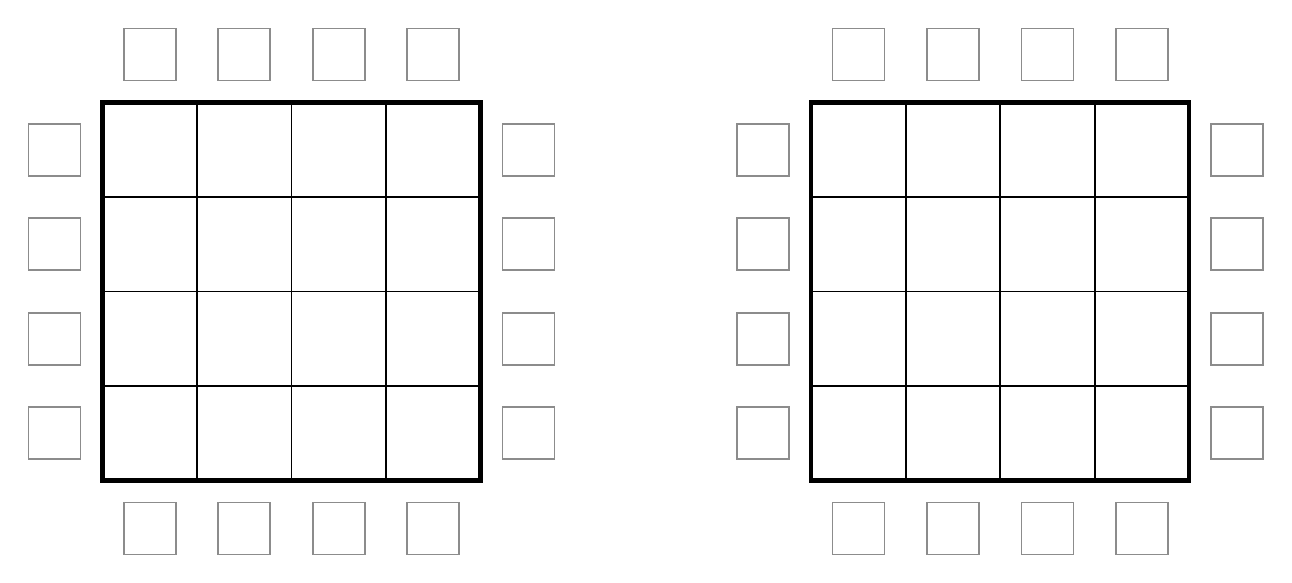
\begin{tikzpicture}
\begin{scope}[shift={(0.000,0.000)}]
\draw[line width=0.7pt] (1.200,0) -- (1.200,4.800);
\draw[line width=0.7pt] (0,1.200) -- (4.800,1.200);
\draw[line width=0.7pt] (2.400,0) -- (2.400,4.800);
\draw[line width=0.7pt] (0,2.400) -- (4.800,2.400);
\draw[line width=0.7pt] (3.600,0) -- (3.600,4.800);
\draw[line width=0.7pt] (0,3.600) -- (4.800,3.600);
\draw[line width=1.6pt] (0,0) rectangle (4.800,4.800);
\draw[black!45, line width=0.6pt] (0.270,5.080) rectangle (0.930,5.740);
\draw[black!45, line width=0.6pt] (1.470,5.080) rectangle (2.130,5.740);
\draw[black!45, line width=0.6pt] (2.670,5.080) rectangle (3.330,5.740);
\draw[black!45, line width=0.6pt] (3.870,5.080) rectangle (4.530,5.740);
\draw[black!45, line width=0.6pt] (0.270,-0.940) rectangle (0.930,-0.280);
\draw[black!45, line width=0.6pt] (1.470,-0.940) rectangle (2.130,-0.280);
\draw[black!45, line width=0.6pt] (2.670,-0.940) rectangle (3.330,-0.280);
\draw[black!45, line width=0.6pt] (3.870,-0.940) rectangle (4.530,-0.280);
\draw[black!45, line width=0.6pt] (-0.940,3.870) rectangle (-0.280,4.530);
\draw[black!45, line width=0.6pt] (-0.940,2.670) rectangle (-0.280,3.330);
\draw[black!45, line width=0.6pt] (-0.940,1.470) rectangle (-0.280,2.130);
\draw[black!45, line width=0.6pt] (-0.940,0.270) rectangle (-0.280,0.930);
\draw[black!45, line width=0.6pt] (5.080,3.870) rectangle (5.740,4.530);
\draw[black!45, line width=0.6pt] (5.080,2.670) rectangle (5.740,3.330);
\draw[black!45, line width=0.6pt] (5.080,1.470) rectangle (5.740,2.130);
\draw[black!45, line width=0.6pt] (5.080,0.270) rectangle (5.740,0.930);
\end{scope}
\begin{scope}[shift={(9.000,0.000)}]
\draw[line width=0.7pt] (1.200,0) -- (1.200,4.800);
\draw[line width=0.7pt] (0,1.200) -- (4.800,1.200);
\draw[line width=0.7pt] (2.400,0) -- (2.400,4.800);
\draw[line width=0.7pt] (0,2.400) -- (4.800,2.400);
\draw[line width=0.7pt] (3.600,0) -- (3.600,4.800);
\draw[line width=0.7pt] (0,3.600) -- (4.800,3.600);
\draw[line width=1.6pt] (0,0) rectangle (4.800,4.800);
\draw[black!45, line width=0.6pt] (0.270,5.080) rectangle (0.930,5.740);
\draw[black!45, line width=0.6pt] (1.470,5.080) rectangle (2.130,5.740);
\draw[black!45, line width=0.6pt] (2.670,5.080) rectangle (3.330,5.740);
\draw[black!45, line width=0.6pt] (3.870,5.080) rectangle (4.530,5.740);
\draw[black!45, line width=0.6pt] (0.270,-0.940) rectangle (0.930,-0.280);
\draw[black!45, line width=0.6pt] (1.470,-0.940) rectangle (2.130,-0.280);
\draw[black!45, line width=0.6pt] (2.670,-0.940) rectangle (3.330,-0.280);
\draw[black!45, line width=0.6pt] (3.870,-0.940) rectangle (4.530,-0.280);
\draw[black!45, line width=0.6pt] (-0.940,3.870) rectangle (-0.280,4.530);
\draw[black!45, line width=0.6pt] (-0.940,2.670) rectangle (-0.280,3.330);
\draw[black!45, line width=0.6pt] (-0.940,1.470) rectangle (-0.280,2.130);
\draw[black!45, line width=0.6pt] (-0.940,0.270) rectangle (-0.280,0.930);
\draw[black!45, line width=0.6pt] (5.080,3.870) rectangle (5.740,4.530);
\draw[black!45, line width=0.6pt] (5.080,2.670) rectangle (5.740,3.330);
\draw[black!45, line width=0.6pt] (5.080,1.470) rectangle (5.740,2.130);
\draw[black!45, line width=0.6pt] (5.080,0.270) rectangle (5.740,0.930);
\end{scope}
\end{tikzpicture}
\end{center}
\end{minipage}
\par\vspace{0.75cm}
\begin{minipage}{\linewidth}\RaggedRight
\prob{7}There are 24 different rows of four towers 1, 2, 3, and 4 cubes tall. Sort them by the two numbers seen from the ends, and write in the table how many rows show each pair.
\vspace*{0.2cm}
\begin{center}
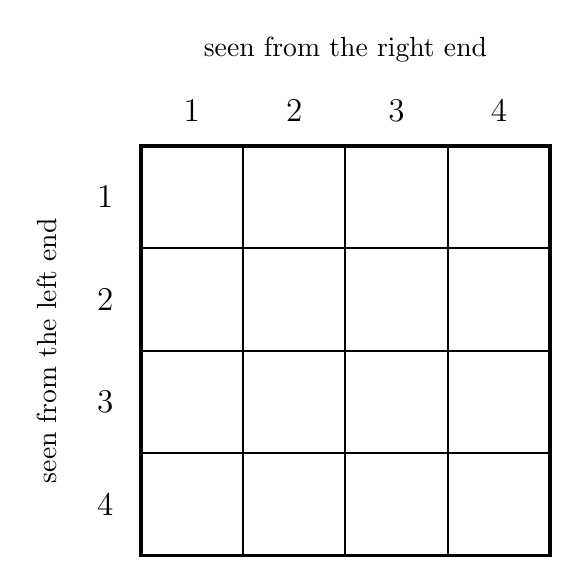
\begin{tikzpicture}
\draw[line width=0.7pt] (0.000,0) -- (0.000,-5.200);
\draw[line width=0.7pt] (0,0.000) -- (5.200,0.000);
\draw[line width=0.7pt] (1.300,0) -- (1.300,-5.200);
\draw[line width=0.7pt] (0,-1.300) -- (5.200,-1.300);
\draw[line width=0.7pt] (2.600,0) -- (2.600,-5.200);
\draw[line width=0.7pt] (0,-2.600) -- (5.200,-2.600);
\draw[line width=0.7pt] (3.900,0) -- (3.900,-5.200);
\draw[line width=0.7pt] (0,-3.900) -- (5.200,-3.900);
\draw[line width=0.7pt] (5.200,0) -- (5.200,-5.200);
\draw[line width=0.7pt] (0,-5.200) -- (5.200,-5.200);
\draw[line width=1.4pt] (0,0) rectangle (5.200,-5.200);
\node at (0.650,0.45) {\large 1};
\node at (-0.45,-0.650) {\large 1};
\node at (1.950,0.45) {\large 2};
\node at (-0.45,-1.950) {\large 2};
\node at (3.250,0.45) {\large 3};
\node at (-0.45,-3.250) {\large 3};
\node at (4.550,0.45) {\large 4};
\node at (-0.45,-4.550) {\large 4};
\node[anchor=south] at (2.600,0.95) {seen from the right end};
\node[anchor=south, rotate=90] at (-0.95,-2.600) {seen from the left end};
\end{tikzpicture}
\end{center}
\end{minipage}
\par\vspace{0.75cm}
\newpage
\begin{minipage}{\linewidth}\RaggedRight
\prob{8}There are 120 different rows of five towers 1, 2, 3, 4, and 5 cubes tall. How many of them show exactly 1 tower from the left end? How many show exactly 2? Explain how you counted.
\vspace*{6.0cm}
\end{minipage}
\par\vspace{0.75cm}
\begin{minipage}{\linewidth}\RaggedRight
\prob{9}Can two different 4-by-4 cities have exactly the same sixteen numbers around them? If they can, find two. If not, explain why.
\vspace*{0.2cm}
\begin{center}
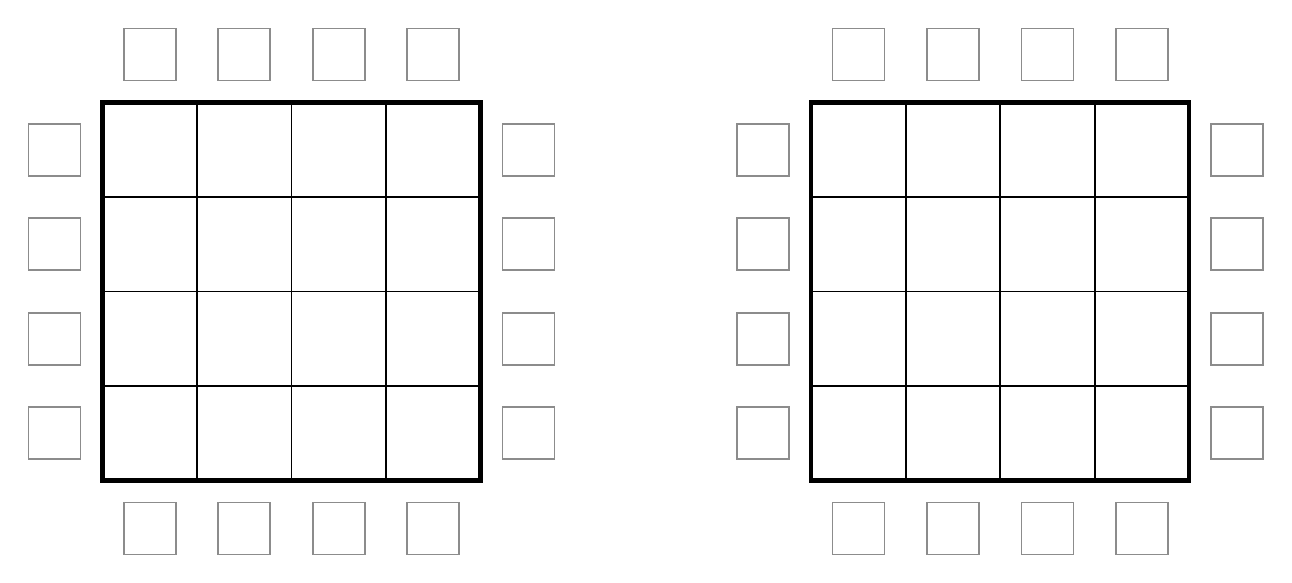
\begin{tikzpicture}
\begin{scope}[shift={(0.000,0.000)}]
\draw[line width=0.7pt] (1.200,0) -- (1.200,4.800);
\draw[line width=0.7pt] (0,1.200) -- (4.800,1.200);
\draw[line width=0.7pt] (2.400,0) -- (2.400,4.800);
\draw[line width=0.7pt] (0,2.400) -- (4.800,2.400);
\draw[line width=0.7pt] (3.600,0) -- (3.600,4.800);
\draw[line width=0.7pt] (0,3.600) -- (4.800,3.600);
\draw[line width=1.6pt] (0,0) rectangle (4.800,4.800);
\draw[black!45, line width=0.6pt] (0.270,5.080) rectangle (0.930,5.740);
\draw[black!45, line width=0.6pt] (1.470,5.080) rectangle (2.130,5.740);
\draw[black!45, line width=0.6pt] (2.670,5.080) rectangle (3.330,5.740);
\draw[black!45, line width=0.6pt] (3.870,5.080) rectangle (4.530,5.740);
\draw[black!45, line width=0.6pt] (0.270,-0.940) rectangle (0.930,-0.280);
\draw[black!45, line width=0.6pt] (1.470,-0.940) rectangle (2.130,-0.280);
\draw[black!45, line width=0.6pt] (2.670,-0.940) rectangle (3.330,-0.280);
\draw[black!45, line width=0.6pt] (3.870,-0.940) rectangle (4.530,-0.280);
\draw[black!45, line width=0.6pt] (-0.940,3.870) rectangle (-0.280,4.530);
\draw[black!45, line width=0.6pt] (-0.940,2.670) rectangle (-0.280,3.330);
\draw[black!45, line width=0.6pt] (-0.940,1.470) rectangle (-0.280,2.130);
\draw[black!45, line width=0.6pt] (-0.940,0.270) rectangle (-0.280,0.930);
\draw[black!45, line width=0.6pt] (5.080,3.870) rectangle (5.740,4.530);
\draw[black!45, line width=0.6pt] (5.080,2.670) rectangle (5.740,3.330);
\draw[black!45, line width=0.6pt] (5.080,1.470) rectangle (5.740,2.130);
\draw[black!45, line width=0.6pt] (5.080,0.270) rectangle (5.740,0.930);
\end{scope}
\begin{scope}[shift={(9.000,0.000)}]
\draw[line width=0.7pt] (1.200,0) -- (1.200,4.800);
\draw[line width=0.7pt] (0,1.200) -- (4.800,1.200);
\draw[line width=0.7pt] (2.400,0) -- (2.400,4.800);
\draw[line width=0.7pt] (0,2.400) -- (4.800,2.400);
\draw[line width=0.7pt] (3.600,0) -- (3.600,4.800);
\draw[line width=0.7pt] (0,3.600) -- (4.800,3.600);
\draw[line width=1.6pt] (0,0) rectangle (4.800,4.800);
\draw[black!45, line width=0.6pt] (0.270,5.080) rectangle (0.930,5.740);
\draw[black!45, line width=0.6pt] (1.470,5.080) rectangle (2.130,5.740);
\draw[black!45, line width=0.6pt] (2.670,5.080) rectangle (3.330,5.740);
\draw[black!45, line width=0.6pt] (3.870,5.080) rectangle (4.530,5.740);
\draw[black!45, line width=0.6pt] (0.270,-0.940) rectangle (0.930,-0.280);
\draw[black!45, line width=0.6pt] (1.470,-0.940) rectangle (2.130,-0.280);
\draw[black!45, line width=0.6pt] (2.670,-0.940) rectangle (3.330,-0.280);
\draw[black!45, line width=0.6pt] (3.870,-0.940) rectangle (4.530,-0.280);
\draw[black!45, line width=0.6pt] (-0.940,3.870) rectangle (-0.280,4.530);
\draw[black!45, line width=0.6pt] (-0.940,2.670) rectangle (-0.280,3.330);
\draw[black!45, line width=0.6pt] (-0.940,1.470) rectangle (-0.280,2.130);
\draw[black!45, line width=0.6pt] (-0.940,0.270) rectangle (-0.280,0.930);
\draw[black!45, line width=0.6pt] (5.080,3.870) rectangle (5.740,4.530);
\draw[black!45, line width=0.6pt] (5.080,2.670) rectangle (5.740,3.330);
\draw[black!45, line width=0.6pt] (5.080,1.470) rectangle (5.740,2.130);
\draw[black!45, line width=0.6pt] (5.080,0.270) rectangle (5.740,0.930);
\end{scope}
\end{tikzpicture}
\end{center}
\vspace*{3.0cm}
\end{minipage}
\par\vspace{0.75cm}
\end{document}
